\documentclass[11pt]{article}

\usepackage[a4paper,margin=1in]{geometry}
\usepackage[T1]{fontenc}
\usepackage{lmodern}
\usepackage{microtype}
\usepackage{amsmath,amssymb,amsthm,mathtools}
\usepackage{booktabs}
\usepackage{array}
\usepackage{longtable}
\usepackage{graphicx}
\usepackage{enumitem}
\usepackage{algorithm}
\usepackage{algpseudocode}
\usepackage{tikz}
\usetikzlibrary{calc,positioning,arrows.meta}
\usepackage[hidelinks]{hyperref}
\usepackage{fancyhdr}
\usepackage{lastpage}
\usepackage{xcolor}
\usepackage{url}
\usepackage{authblk}

\hypersetup{
  pdftitle={Weak Saturation of the 3-Cube in Complete Graphs: Exact Values at Orders 9, 10, 11},
  pdfauthor={Vedansh Saha, Nipun Saha},
  pdfsubject={Weak saturation of the three-dimensional cube in complete graphs},
  pdfkeywords={weak saturation, graph bootstrap percolation, hypercube, extremal graph theory, finite closure systems}
}

\setlength{\headheight}{14pt}
\setlength{\emergencystretch}{5em}
\setlist{nosep}
\numberwithin{equation}{section}

\newtheorem{theorem}{Theorem}[section]
\newtheorem{proposition}[theorem]{Proposition}
\newtheorem{lemma}[theorem]{Lemma}
\newtheorem{corollary}[theorem]{Corollary}
\newtheorem{definition}[theorem]{Definition}
\newtheorem{remark}[theorem]{Remark}

\newcommand{\wsat}{\operatorname{wsat}}
\newcommand{\cl}{\operatorname{cl}}
\newcommand{\Aut}{\operatorname{Aut}}
\newcommand{\Stab}{\operatorname{Stab}}
\newcommand{\Q}{Q_3}
\newcommand{\U}{U}
\newcommand{\GammaG}{\Gamma}
\newcommand{\E}{E}
\newcommand{\V}{V}
\newcommand{\ed}[2]{#1#2}
\newcommand{\phiMap}{\varphi}

\definecolor{seedblue}{RGB}{36,97,186}
\definecolor{markedred}{RGB}{190,55,42}
\definecolor{activationgreen}{RGB}{35,135,76}
\definecolor{backgray}{RGB}{125,125,125}
\definecolor{outsideorange}{RGB}{244,218,177}
\definecolor{facegray}{RGB}{226,233,243}

\graphicspath{{figures/}}

\pagestyle{fancy}
\fancyhf{}
\fancyhead[L]{Weak saturation of the 3-cube in complete graphs}
\fancyhead[R]{\thepage\,/\,\pageref{LastPage}}
\renewcommand{\headrulewidth}{0.4pt}

\title{\textbf{Weak Saturation of the 3-Cube in Complete Graphs:\\ Exact Values at Orders 9, 10, 11}}
\author[1]{Vedansh Saha, Nipun Saha}
\affil[1]{Dhirubhai Ambani International School, Mumbai}

\begin{document}
\maketitle

\begin{abstract}
Let $Q_3$ be the three-dimensional cube. The weak saturation number of $Q_3$ in complete graphs is determined exactly at three consecutive orders:
\[
\wsat(K_9,Q_3)=16,\qquad
\wsat(K_{10},Q_3)=18,\qquad
\wsat(K_{11},Q_3)=19.
\]
The value at $n=9$ gives a counterexample to the formula $\wsat(K_n,Q_3)=2n-1$ reported as a conjecture in the 2025 Park City Mathematics Institute project slides of Trakulthongchai, Xu, and Zhu. The $n=9$ result is established by an exact closure computation: after normalizing the first edge of a saturation order, the problem becomes the search for minimum generating sets in a monotone closure system on the $\binom92-12=24$ edges outside a fixed cube. All $\binom{24}{4}=10,626$ four-edge seeds are excluded, while a five-edge seed percolates. An independent Go implementation uses explicit edge lists and queue-indexed implications and reproduces the lower bound. A separate graph-level verifier enumerates all $7,560$ labelled copies of $Q_3$ in $K_9$ and checks the complete certificate.

For $n=10$, all $\binom{33}{6}=1,107,568$ six-edge seeds are reduced by the stabilizer of the marked cube edge to $146,131$ orbit representatives, none of which percolates. For $n=11$, the seven-edge orbit layer contains $1,498,208$ representatives; none percolates. Burnside's lemma independently gives the $n=11$ orbit counts. Explicit certificates of sizes $16$, $18$, and $19$ provide the matching upper bounds. The certificate tables record, for every edge addition, an injective vertex map from the canonical cube and the earlier additions used by the witness. A structural analysis of the $n=10$ certificate isolates a twin-vertex activation lemma and three cube switches. The general clique-extension construction then gives $\wsat(K_n,Q_3)\le 2n-3$ for every $n\ge11$.
\end{abstract}

\noindent\textbf{Keywords:} weak saturation; graph bootstrap percolation; hypercube; extremal graph theory; finite closure systems; computer-assisted proof.

\section{Introduction}
Let $H$ and $G$ be finite graphs with $H\subseteq G$. A spanning subgraph $F\subseteq G$ is \emph{weakly $H$-saturated in $G$} if the edges of $G\setminus F$ can be ordered as $e_1,\ldots,e_t$ so that, for every $i$, the graph
\[
F+e_1+\cdots+e_i
\]
contains a copy of $H$ in which $e_i$ is an edge. The weak saturation number is
\[
\wsat(G,H)=\min\{|E(F)|:F\text{ is weakly }H\text{-saturated in }G\}.
\]
For complete hosts, write $\wsat(n,H)=\wsat(K_n,H)$. The parameter originates with Bollob\'as \cite{Bollobas1968} and has connections with bootstrap percolation, extremal graph theory, and linear-algebraic methods \cite{Balogh2012,MNS2017,KMM2021}.

The problem studied here is
\[
\boxed{\text{Determine }\wsat(K_n,Q_3)\text{ for }n\ge 8.}
\]
The cube has $8$ vertices, $12$ edges, and minimum degree $3$. The quantity $\wsat(K_n,Q_3)$ is currently listed as an open problem in the Open Problem Garden \cite{OPG}. The 2025 PCMI project slides of Trakulthongchai, Xu, and Zhu state the bound $\wsat(K_n,Q_3)\le 2n-1$ for $n\ge8$, report the values $15$ and $17$ at $n=8$ and $n=9$, and conjecture equality with $2n-1$ \cite{PCMI2025}. The $n=9$ case is re-evaluated from the closure system defined below. The exact scan of all $\binom{24}{4}=10,626$ normalized four-edge seeds gives no percolating seed, while a five-edge certificate percolates. An independent Go implementation with explicit edge lists and queue-based activation gives the same four-edge exclusion, and a separate graph-level verifier checks the certificate against all $7,560$ labelled copies of $Q_3$ in $K_9$. Consequently, $\wsat(K_9,Q_3)=16$.

\begin{theorem}[Main result]\label{thm:main}
\[
\boxed{\wsat(K_9,Q_3)=16,\qquad \wsat(K_{10},Q_3)=18,\qquad \wsat(K_{11},Q_3)=19.}
\]
\end{theorem}

The proof separates the finite generating-set problem from the graph-theoretic bookkeeping. The first-edge normalization supplies a fixed cube core. The closure operator records all legal outside-edge additions. Its finite fixed-point computation is proved correct, and the symmetry reductions are proved complete. The upper bounds are verified edge by edge by explicit cube embeddings.

\section{Preliminaries and known bounds}\label{sec:prelim}

\subsection{The cube}
Identify $V(Q_3)$ with $\mathbb F_2^3$, written as $\{0,1,\ldots,7\}$ in binary order. Thus
\[
xy\in E(Q_3)\iff x\oplus y\text{ has Hamming weight }1.
\]
Consequently
\[
|V(Q_3)|=8,\qquad |E(Q_3)|=12,\qquad \delta(Q_3)=3.
\]
Edges are written as concatenated endpoint labels; when the vertex $10$ occurs, a thin space separates the labels, so $0\,10$ denotes the edge $\{0,10\}$.

The automorphism group has order
\[
|\Aut(Q_3)|=2^3\cdot 3!=48,
\]
and $\Aut(Q_3)$ is transitive on the twelve cube edges.

\begin{lemma}[Minimum degree]\label{lem:mindeg}
Let $H$ be a graph with minimum degree $\delta(H)\ge2$. If $F$ is weakly $H$-saturated in $K_n$, then
\[
\delta(F)\ge \delta(H)-1.
\]
In particular, every weakly $Q_3$-saturated spanning graph has minimum degree at least $2$.
\end{lemma}

\begin{proof}
Suppose that $v\in V(K_n)$ has $d_F(v)\le \delta(H)-2$. Before the first added edge incident with $v$, the degree of $v$ is still at most $\delta(H)-2$. If an edge incident with $v$ were added at that stage and completed a copy of $H$, the image of $v$ in that copy would have at least $\delta(H)$ incident edges, while only the newly added edge can increase the degree of $v$. Hence such an addition is impossible. Therefore no edge incident with $v$ can ever be added, contradicting saturation.
\end{proof}

\subsection{Analytic lower bounds and asymptotic scale}
For a graph $H$ with $v$ vertices, $\ell$ edges, and minimum degree $\delta>1$, Terekhov and Zhukovskii proved the following lower bound \cite{TZ2025}:
\[
\wsat(K_n,H)\ge
\begin{cases}
\dfrac{\delta}{2}(n-v)+\ell-1,& H\text{ is 2-edge-connected},\\
\left\lceil\left(\dfrac{\delta}{2}-\dfrac{1}{\delta+1}\right)(n-v)\right\rceil+\ell-1,&\text{in general.}
\end{cases}
\tag{2.1}
\]
Since $Q_3$ is 2-edge-connected,
\[
\wsat(K_n,Q_3)\ge \frac32(n-8)+11.
\tag{2.2}
\]
For the invariant used in their sharper theorem, set
\[
e_i=\min_{\substack{S\subseteq V(Q_3)\\|S|=i}}
\left(|E(Q_3)|-|E(Q_3-S)|-1\right),
\qquad 1\le i\le7.
\tag{2.3}
\]
A direct calculation gives
\[
\begin{array}{c|ccccccc}
i&1&2&3&4&5&6&7\\ \hline
e_i&2&4&6&7&9&10&11\\
\end{array}
\tag{2.4}
\]
and hence
\[
\min_{1\le i\le7}\frac{e_i}{i}=\frac{11}{7}.
\tag{2.5}
\]
The maximal subadditive function in Theorem~2.1 of \cite{TZ2025} is obtained from the values $e_i$ by
\[
g^*(0)=0,\qquad
g^*(t)=\min_{\substack{s\ge1,\ i_1,\ldots,i_s\in\{1,\ldots,7\}\\ i_1+\cdots+i_s=t}}
\bigl(e_{i_1}+\cdots+e_{i_s}\bigr).
\tag{2.6}
\]
In particular, $g^*(1)=2$, $g^*(2)=4$, and $g^*(3)=6$.

The calculation behind (2.4) follows from the induced-edge maxima in the cube. Let
\[
m_i=\max_{|S|=i}|E(Q_3[S])|.
\]
Since every vertex of $S$ has degree $3$ in $Q_3$,
\[
|E(Q_3)|-|E(Q_3-S)|=3i-|E(Q_3[S])|=3i-m_i.
\]
Therefore $e_i=3i-m_i-1$. The required maxima are
\[
\begin{array}{c|ccccccc}
i&1&2&3&4&5&6&7\\ \hline
m_i&0&1&2&4&5&7&9\\
\end{array}
\]
and are attained, for example, by the sets
\[
\{0\},\ \{0,1\},\ \{0,1,2\},\ \{0,1,2,3\},\ \{0,1,2,3,4\},\ \{0,1,2,3,4,5\},\ V(Q_3)\setminus\{7\},
\]
respectively. Substitution yields the values in (2.4).

Theorem 2.1 of \cite{TZ2025}, together with the existence of the asymptotic weak saturation slope proved by Alon \cite{Alon1985}, therefore gives
\[
\frac{11}{7}\le c_{Q_3}:=\lim_{n\to\infty}\frac{\wsat(K_n,Q_3)}{n}\le 2.
\tag{2.7}
\]
The upper bound in (2.7) comes from the standard clique-extension construction. The values established here are finite exact values inside this asymptotic interval; (2.2)--(2.6) do not determine $\wsat(K_9,Q_3)$.

\section{A finite closure system}\label{sec:closure}

\subsection{Marked cube and outside edges}
Fix the canonical cube
\[
C=Q_3[\{0,1,\ldots,7\}]
\]
and the marked edge
\[
e^*=01.
\]
For $n\ge8$ let
\[
U_n=E(K_n)\setminus E(C),
\qquad |U_n|=\binom n2-12.
\tag{3.1}
\]
Every weak saturation order can be normalized so that the first edge is $e^*$.

\begin{lemma}[First-edge normalization]\label{lem:first}
Let $F$ be weakly $Q_3$-saturated in $K_n$, and let $e$ be the first edge in a
legal addition order. There is a relabelling of $V(K_n)$ under which
\[
e=e^*,\qquad e^*\notin F,\qquad E(C)\setminus\{e^*\}\subseteq F,
\]
and every edge of $F$ outside $E(C)$ belongs to $U_n$.
\end{lemma}

\begin{proof}
The first edge $e$ is absent from $F$ and completes a copy $Q$ of $Q_3$ whose
other eleven edges lie in $F$. Since $\Aut(Q_3)$ is edge-transitive, there is
an isomorphism of the marked pair $(Q,e)$ with $(C,e^*)$. Extend this
isomorphism to a permutation of $V(K_n)$. Under the resulting relabelling,
$e=e^*$ and $E(C)\setminus\{e^*\}\subseteq F$. Every remaining edge of $F$
lies outside $E(C)$ and hence belongs to $U_n$.
\end{proof}

\begin{definition}[Outside closure]\label{def:closure}
For $S\subseteq U_n$, the closure $\cl_n(S)$ is the least subset $T\subseteq U_n$ satisfying $S\subseteq T$ and the following implication: if $Q\subseteq K_n$ is a copy of $Q_3$, $e\in E(Q)\cap U_n$, and
\[
(E(Q)\cap U_n)\setminus\{e\}\subseteq T,
\]
then $e\in T$.
\end{definition}

For a copy $Q$ of $Q_3$, put
\[
M(Q)=E(Q)\cap U_n.
\]
The copy contributes the implications
\[
M(Q)\setminus\{e\}\longrightarrow e,
\qquad e\in M(Q).
\tag{3.2}
\]
Copies with the same outside set $M(Q)$ produce the same implications and can be merged.

\begin{algorithm}[t]
\caption{Exact closure computation}
\label{alg:closure}
\begin{algorithmic}[1]
\Require seed $S\subseteq U_n$ and the distinct outside masks $\mathcal M_n=\{M(Q):Q\cong Q_3\}$
\Ensure $T=\cl_n(S)$
\State $T\gets S$
\State insert into $T$ every target of an implication with empty antecedent, and enqueue the inserted edges
\State enqueue every edge of $S$
\State maintain, for each implication $A\to e$, the number of edges of $A$ already in $T$
\While{the queue is nonempty}
    \State remove an edge $f$ from the queue
    \ForAll{implications $A\to e$ with $f\in A$}
        \State increment the counter for $A\to e$
        \If{all edges of $A$ are in $T$ and $e\notin T$}
            \State add $e$ to $T$ and enqueue $e$
        \EndIf
    \EndFor
\EndWhile
\State \Return $T$
\end{algorithmic}
\end{algorithm}

\begin{lemma}[Correctness of Algorithm~\ref{alg:closure}]\label{lem:closure}
Algorithm~\ref{alg:closure} terminates and returns $\cl_n(S)$.
\end{lemma}

\begin{proof}
Let $T_j$ denote the value of $T$ after $j$ successful insertions. We show by
induction that $T_j\subseteq\cl_n(S)$. This holds for $j=0$ because
$S\subseteq\cl_n(S)$. If an edge $e$ is inserted at step $j+1$, then some
rule $A\to e$ has $A\subseteq T_j$. By the induction hypothesis,
$A\subseteq\cl_n(S)$, so the defining closure property gives
$e\in\cl_n(S)$. Hence every edge inserted by the algorithm lies in
$\cl_n(S)$.

At most $|U_n|$ edges can be inserted, so the algorithm terminates. At
termination, if $A\to e$ is any closure rule with $A\subseteq T$, then the
counter for that rule has reached $|A|$ and the target $e$ has been inserted.
Thus $T$ is closed under all rules defining $\cl_n(S)$. Since $S\subseteq T$,
minimality of $\cl_n(S)$ gives $\cl_n(S)\subseteq T$. Therefore
$T=\cl_n(S)$.
\end{proof}



\begin{lemma}[Certificate criterion]\label{lem:certificate}
Let $F_0\subseteq K_n$ and let $e_1,\ldots,e_t$ be the missing edges of $F_0$. Suppose that for each $i$ there is an injective map $\phi_i:V(Q_3)\to V(K_n)$ satisfying
\[
\phi_i(0)\phi_i(1)=e_i
\]
and
\[
\phi_i(E(Q_3)\setminus\{01\})\subseteq E(F_0)\cup\{e_1,\ldots,e_{i-1}\}.
\]
Then $F_0$ is weakly $Q_3$-saturated in $K_n$.
\end{lemma}

\begin{proof}
For each $i$, injectivity of $\phi_i$ makes its image a copy of $Q_3$. The displayed containment shows that every edge of this copy except $e_i$ is present immediately before step $i$. Hence adding $e_i$ creates a copy of $Q_3$. Applying this argument successively proves that the sequence is legal and ends with $K_n$.
\end{proof}

\begin{lemma}[Sequential equivalence]\label{lem:seq}
For $S\subseteq U_n$,
\[
(C-e^*)\cup S\text{ is weakly $Q_3$-saturated in }K_n
\quad\Longleftrightarrow\quad
\cl_n(S)=U_n.
\]
\end{lemma}

\begin{proof}
Suppose that $(C-e^*)\cup S$ is weakly $Q_3$-saturated. Let
$e_1,\ldots,e_t$ be a legal order. By Lemma~\ref{lem:first}, after a
relabelling the first edge completes $C$ and is $e^*$. Moving $e^*$ to the
front preserves legality because an edge already available at a given stage
remains available after additional edges have been added. Delete this first
edge from the order.

Consider an edge $e_i\in U_n$ in the resulting order. Its witnessing cube
$Q_i$ has every edge other than $e_i$ present when $e_i$ is added. The edges of
$Q_i$ that lie in $U_n$ therefore satisfy one of the implications (3.2).
Induction on the order position shows that every outside edge added by the
saturation process belongs to $\cl_n(S)$. The final graph is $K_n$, so
$\cl_n(S)=U_n$.

Conversely, suppose that $\cl_n(S)=U_n$. Define rounds by
$T_0=S$ and
\[
T_{r+1}=T_r\cup\{e\in U_n:\exists Q\cong Q_3,
M(Q)\setminus\{e\}\subseteq T_r\}.
\]
The sequence stabilizes because $U_n$ is finite. Add $e^*$ first. For
$e\in T_{r+1}\setminus T_r$, its witnessing cube has all other outside
edges in $T_r$, while all cube edges outside $U_n$ lie in $E(C)$ and are
present after $e^*$ is added. Thus each edge in a round is legally addable
once all earlier rounds have been added. Serializing the rounds gives a legal
weak $Q_3$-saturation order.
\end{proof}

\begin{lemma}[Seed identity]\label{lem:seed}
Let
\[
\sigma_n=\min\{|S|:S\subseteq U_n,\ \cl_n(S)=U_n\}.
\]
Then
\[
\boxed{\wsat(K_n,Q_3)=11+\sigma_n.}
\tag{3.3}
\]
\end{lemma}

\begin{proof}
Lemma~\ref{lem:first} puts eleven cube edges in every normalized initial graph. The remaining initial edges form a seed $S\subseteq U_n$. Lemma~\ref{lem:seq} shows that $S$ must percolate, so every weak saturation graph has at least $11+\sigma_n$ edges. Conversely, a percolating seed together with $C-e^*$ gives a weak saturation graph with $11+|S|$ initial edges. Minimizing over $S$ proves (3.3).
\end{proof}

\begin{lemma}[Monotonicity]\label{lem:mono}
If $S\subseteq T\subseteq U_n$, then
\[
\cl_n(S)\subseteq\cl_n(T).
\]
Hence every superset of a percolating seed also percolates.
\end{lemma}

\begin{proof}
The defining implications of the closure system are monotone in the current edge set. An induction on closure rounds gives the inclusion.
\end{proof}

\subsection{Enumeration of the closure rules}\label{sec:maskenumeration}
For each $n$, construct the closure rules by enumerating all copies of $Q_3$
in $K_n$. Choose an $8$-vertex subset $W\subseteq V(K_n)$ and enumerate the
edge sets on $W$ isomorphic to $Q_3$. For a copy $Q$, retain only the edges
outside the fixed cube,
\[
M(Q)=E(Q)\cap U_n.
\]
The copy yields the implications
\[
M(Q)\setminus\{e\}\longrightarrow e,
\qquad e\in M(Q).
\tag{3.4}
\]
If two cube copies have the same outside mask, their implications coincide,
so the two copies can be merged for closure computation.

The number of labelled cube copies is
\[
N_n=\binom{n}{8}\frac{8!}{|\Aut(Q_3)|},
\tag{3.5}
\]
which gives
\[
N_9=7,560,\qquad N_{10}=37,800,\qquad N_{11}=138,600.
\tag{3.6}
\]
The corresponding numbers of distinct outside masks are
\[
7,122,\qquad36,506,\qquad135,650.
\tag{3.7}
\]

\begin{algorithm}[t]
\caption{Construction of the complete outside-rule system}
\label{alg:masks}
\begin{algorithmic}[1]
\Require $n\ge8$
\Ensure distinct outside masks $\mathcal M_n$
\State $\mathcal M_n\gets\varnothing$
\ForAll{$W\in\binom{V(K_n)}8$}
    \ForAll{cube edge sets on $W$ isomorphic to $Q_3$}
        \State compute $M(Q)=E(Q)\cap U_n$
        \State insert $M(Q)$ into $\mathcal M_n$
    \EndFor
\EndFor
\State \Return $\mathcal M_n$
\end{algorithmic}
\end{algorithm}

\begin{lemma}[Completeness of the mask system]\label{lem:masks}
Algorithm~\ref{alg:masks} produces every implication required by
Definition~\ref{def:closure}.
\end{lemma}

\begin{proof}
Every copy $Q\cong Q_3$ in $K_n$ is generated on its $8$-vertex set, so its
outside mask occurs in $\mathcal M_n$. Conversely, every stored mask is the
outside mask of a cube copy. The twelve edges of that cube that lie outside
$U_n$ belong to $E(C)$, and after $e^*$ is added they are already present.
Thus the legality of an outside edge depends on the cube only through
$M(Q)$, and merging equal masks preserves the complete implication system.
\end{proof}

\subsection{Symmetry reduction}
Define
\[
\Gamma_n=
\Stab_{\Aut(Q_3)}(e^*)\times S_{\{8,\ldots,n-1\}},
\tag{3.4}
\]
where the first factor acts on $\{0,\ldots,7\}$ and the second factor permutes the vertices outside the cube. Since an edge orbit of $\Aut(Q_3)$ has size $12$,
\[
|\Stab_{\Aut(Q_3)}(e^*)|=48/12=4,
\]
so
\[
|\Gamma_9|=4,\qquad |\Gamma_{10}|=8,\qquad |\Gamma_{11}|=24.
\tag{3.5}
\]

\begin{definition}[Canonical orbit representative]\label{def:can}
Fix an ordering of $U_n$ and encode each subset of $U_n$ by its binary incidence
mask. Define
\[
\operatorname{can}(S)=\min\{gS:g\in\Gamma_n\},
\tag{3.8}
\]
where the minimum is taken in the induced lexicographic order.
\end{definition}

\begin{lemma}[Equivariance]\label{lem:equiv}
For every $g\in\Gamma_n$ and $S\subseteq U_n$,
\[
\cl_n(gS)=g\cl_n(S).
\]
\end{lemma}

\begin{proof}
If $A\to e$ is induced by a cube $Q$, then $gA\to ge$ is induced by the
cube $gQ$. Hence $g$ preserves the implication system. Induction over the
closure rounds gives the stated identity.
\end{proof}

\begin{lemma}[Canonicalization criterion]\label{lem:can}
For $S,T\subseteq U_n$,
\[
\operatorname{can}(S)=\operatorname{can}(T)
\quad\Longleftrightarrow\quad
T=gS\text{ for some }g\in\Gamma_n.
\]
\end{lemma}

\begin{proof}
If $T=gS$, then $S$ and $T$ have the same orbit and therefore the same
canonical representative. Conversely, if the canonical representatives
agree, choose $g,h\in\Gamma_n$ with $gS=hT$. Then
$T=h^{-1}gS$.
\end{proof}

By Lemmas~\ref{lem:equiv} and~\ref{lem:can}, percolation and closure size are
constant on each orbit, so one representative from each orbit suffices.

\begin{algorithm}[t]
\caption{Complete generation of the next orbit layer}
\label{alg:orbits}
\begin{algorithmic}[1]
\Require representatives $\mathcal R_k$ of all $\Gamma_n$-orbits on $k$-subsets
\Ensure representatives $\mathcal R_{k+1}$ of all $\Gamma_n$-orbits on $(k+1)$-subsets
\State $\mathcal C\gets\varnothing$
\ForAll{$R\in\mathcal R_k$}
    \ForAll{$e\in U_n\setminus R$}
        \State insert $\operatorname{can}(R\cup\{e\})$ into $\mathcal C$
    \EndFor
\EndFor
\State deduplicate $\mathcal C$
\State \Return $\mathcal C$
\end{algorithmic}
\end{algorithm}

\begin{lemma}[Layered orbit generation]\label{lem:layer}
Let $\mathcal R_k$ contain one representative from every $\Gamma_n$-orbit of $k$-subsets of $U_n$. The following procedure produces a complete set of representatives for the $(k+1)$-subsets:
\[
\{\operatorname{can}(R\cup\{e\}):R\in\mathcal R_k,\ e\in U_n\setminus R\},
\tag{3.6}
\]
followed by deduplication.
\end{lemma}

\begin{proof}
Let $S$ be any $(k+1)$-subset of $U_n$. Choose $e\in S$ and put $R=S\setminus\{e\}$. By completeness of $\mathcal R_k$, some $g\in\Gamma_n$ maps $R$ to its representative $R_0\in\mathcal R_k$. Then $gS=R_0\cup\{ge\}$ occurs in (3.6), so the orbit of $S$ is represented among the generated candidates.
\end{proof}

\section{\texorpdfstring{The exact value at $n=9$}{The exact value at n=9}}\label{sec:n9}

\subsection{Upper bound}
The seed is
\[
S_9=\{03,05,08,12,28\},
\tag{4.1}
\]
and the initial graph is
\[
E(F_9)=E(C)\setminus\{01\}\cup S_9.
\tag{4.2}
\]
Explicitly,
\[
\begin{aligned}
E(F_9)=\{&02,03,04,05,08,12,13,15,23,26,28,37,\\
&45,46,57,67\}.
\end{aligned}
\]
The twenty missing edges are added in the order
\[
\begin{array}{llllllllll}
01,&14,&48,&78,&06,&16,&17,&18,&24,&25,\\
27,&34,&35,&36,&38,&47,&56,&58,&68,&07.
\end{array}
\tag{4.3}
\]

\begin{proposition}\label{prop:n9upper}
The graph $F_9$ is weakly $Q_3$-saturated in $K_9$. Hence
\[
\wsat(K_9,Q_3)\le16.
\]
\end{proposition}

\begin{proof}
Apply Lemma~\ref{lem:certificate} to the sequence (4.3). For every row of the $n=9$ witness table in Appendix~\ref{app:witness}, the listed map $\phi_i$ is injective, sends the canonical edge $01$ to the edge added at step $i$, and maps the other eleven cube edges to initial edges or edges appearing in the dependency column. Hence every row certifies a legal addition.

For step $2$, for example,
\[
(\phi_2(0),\ldots,\phi_2(7))=(1,4,0,5,2,6,3,7),
\]
and
\[
\phi_2(E(Q_3))=\{14,01,12,45,46,05,03,57,26,23,67,37\}.
\]
Before step $2$, the edge $01$ was added at step $1$, while the remaining ten non-target edges in this set belong to $E(F_9)$. Thus $14$ is legal. The same finite check applies to all twenty rows. The sequence contains every edge outside $E(F_9)$ exactly once, so the terminal graph is $K_9$.
\end{proof}

The closure rounds for the seed $S_9$ have sizes $5,2,4,12,1$:
\[
\begin{array}{c|l}
\text{round}&\text{edges activated}\\ \hline
0&03,05,08,12,28\\
1&14,48\\
2&16,17,18,78\\
3&06,07,24,25,27,34,35,36,38,47,56,58\\
4&68.
\end{array}
\tag{4.4}
\]
This round decomposition is obtained directly from the implication system and gives a second serialization of the same certificate.

\begin{figure}[t]
\centering
\resizebox{0.72\linewidth}{!}{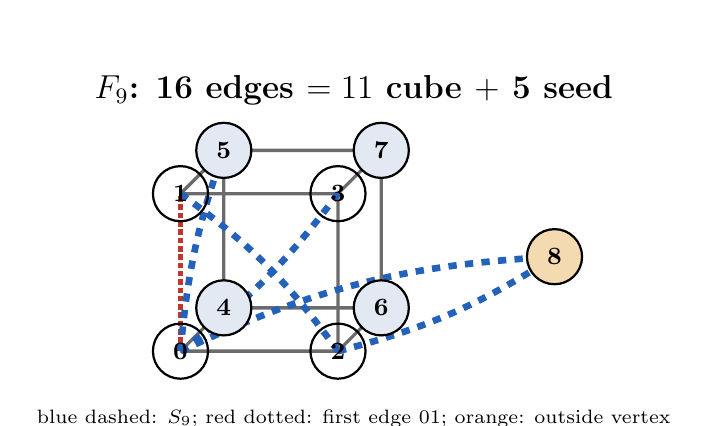
\begin{tikzpicture}[x=1cm,y=1cm,>=Latex]
  \tikzset{
    v/.style={circle,draw=black,thick,minimum size=7mm,inner sep=0pt,font=\small\bfseries},
    back/.style={v,fill=facegray},
    outside/.style={v,fill=outsideorange},
    core/.style={draw=black!58,line width=1.2pt},
    seed/.style={draw=seedblue,line width=2.4pt,dashed},
    marked/.style={draw=markedred,line width=2.0pt,densely dotted},
  }
  \coordinate (v0) at (0,0);
  \coordinate (v1) at (0,2);
  \coordinate (v2) at (2,0);
  \coordinate (v3) at (2,2);
  \coordinate (v4) at (0.55,0.55);
  \coordinate (v5) at (0.55,2.55);
  \coordinate (v6) at (2.55,0.55);
  \coordinate (v7) at (2.55,2.55);
  \coordinate (v8) at (4.75,1.20);

  \draw[core] (v0)--(v2) (v0)--(v4) (v1)--(v3) (v1)--(v5)
              (v2)--(v3) (v2)--(v6) (v3)--(v7)
              (v4)--(v5) (v4)--(v6) (v5)--(v7) (v6)--(v7);
  \draw[marked] (v0)--(v1);

  \draw[seed] (v0) to[bend right=8] (v3);
  \draw[seed] (v0) to[bend left=7] (v5);
  \draw[seed] (v0) to[bend left=11] (v8);
  \draw[seed] (v1) to[bend left=9] (v2);
  \draw[seed] (v2) to[bend right=9] (v8);

  \node[v] at (v0) {0}; \node[v] at (v1) {1};
  \node[v] at (v2) {2}; \node[v] at (v3) {3};
  \node[back] at (v4) {4}; \node[back] at (v5) {5};
  \node[back] at (v6) {6}; \node[back] at (v7) {7};
  \node[outside] at (v8) {8};

  \node[font=\large\bfseries,anchor=south] at (2.2,3.0) {$F_9$: 16 edges $=11$ cube $+$ 5 seed};
  \node[font=\scriptsize,anchor=north] at (2.2,-0.62) {blue dashed: $S_9$; red dotted: first edge $01$; orange: outside vertex};
\end{tikzpicture}
}
\caption{The $n=9$ upper-bound certificate. Solid edges are the eleven canonical cube edges initially present; the red dotted edge is the marked first edge $01$; blue dashed edges form the five-edge seed $S_9$; the orange vertex lies outside the canonical cube.}
\label{fig:n9seed}
\end{figure}

\subsection{Lower bound}
Here
\[
|U_9|=\binom92-12=24.
\]
A weak saturation number at most $15$ would, by (3.3), give a percolating seed of size at most $4$. By Lemma~\ref{lem:mono}, it suffices to exclude four-edge seeds, since every seed of size at most $4$ is contained in a four-edge seed and percolation is monotone.

\begin{proposition}\label{prop:n9lower}
No four-edge subset of $U_9$ percolates. Consequently,
\[
\sigma_9\ge5.
\]
\end{proposition}

\begin{proof}
There are exactly $\binom{24}{4}=10,626$ labelled four-edge subsets of $U_9$. The primary C++ enumeration visits each subset exactly once. Burnside's lemma gives $2,826$ orbits under the order-$4$ group $\Gamma_9$; the $n=9$ lower-bound scan does not use this quotient. For each seed, Algorithm~\ref{alg:closure} computes its exact closure. Every terminal closure has fewer than $24$ edges; the largest has $16$ edges. Therefore no four-edge seed satisfies $\cl_9(S)=U_9$.

The same four-edge exclusion was recomputed by the independent Go implementation in the supplementary folder. That program constructs the $7,560$ labelled cube copies from explicit sorted edge lists, generates the corresponding closure implications, and evaluates the $10,626$ seeds with a queue-based activation routine. It returns zero percolating seeds and maximum closure size $16$.
\end{proof}

The primary exact scan also evaluates the full five-edge layer. Among the $42,504$ five-edge seeds, exactly $6,864$ percolate. Together with the explicit five-edge certificate, this gives $\sigma_9=5$.

The certificate itself was checked at the graph level against every labelled copy of $Q_3$ in $K_9$. The number of distinct labelled cube edge sets is
\[
\frac{\binom98\,8!}{|\Aut(Q_3)|}=\frac{9\cdot40320}{48}=7,560.
\tag{4.5}
\]
The initial graph contains none of these $7,560$ cubes. Each witness row is verified as one of these labelled cube copies, with its eleven non-target edges present at the required stage, and the final graph is $K_9$. This check is implemented separately in \path{supplement/programs/n9_graph_level_check.py}.

\begin{theorem}\label{thm:n9}
\[
\boxed{\wsat(K_9,Q_3)=16.}
\]
\end{theorem}

\begin{proof}
Proposition~\ref{prop:n9upper} gives $\wsat(K_9,Q_3)\le16$, while Proposition~\ref{prop:n9lower} and (3.3) give $\sigma_9\ge5$ and hence $\wsat(K_9,Q_3)\ge16$.
\end{proof}

\begin{corollary}\label{cor:n9family}
For every $n\ge9$,
\[
\wsat(K_n,Q_3)\le2n-2.
\]
Hence $\wsat(K_n,Q_3)=2n-1$ cannot hold for any $n\ge9$.
\end{corollary}

\begin{proof}
Apply Proposition~\ref{prop:extension} repeatedly to the $16$-edge
construction at $n=9$. Each extension adds two initial edges, giving
\[
\wsat(K_n,Q_3)\le16+2(n-9)=2n-2.
\]
\end{proof}

\section{\texorpdfstring{The exact value at $n=10$}{The exact value at n=10}}\label{sec:n10}

\subsection{Upper bound}
The seven-edge seed is
\[
S_{10}=\{12,19,29,35,36,68,78\}.
\tag{5.1}
\]
Together with $C-01$, this gives $18$ initial edges. One legal saturation order is
\[
\begin{array}{cccccccccc}
01,&39,&07,&17,&03,&25,&47,&16,&27,&56,\\
24,&34,&05,&06,&14,&59,&49,&69,&09,&79,\\
28,&58,&18,&38,&48,&08,&89.
\end{array}
\tag{5.2}
\]
The full witness table is in Appendix~\ref{app:witness}.

\begin{proposition}\label{prop:n10upper}
The graph defined by (5.1) is weakly $Q_3$-saturated in $K_{10}$. Hence
\[
\wsat(K_{10},Q_3)\le18.
\]
\end{proposition}

\begin{proof}
Lemma~\ref{lem:certificate} applies to the order (5.2). For each $i$, the witness table gives an injective map $\phi_i:V(Q_3)\to V(K_{10})$ with $\phi_i(0)\phi_i(1)=e_i$ and with every other image of a cube edge belonging to the initial graph or to an earlier step. Hence $e_i$ is legal. The $27$ listed additions are exactly the edges missing from the $18$-edge initial graph, so the terminal graph is $K_{10}$.
\end{proof}

\begin{figure}[t]
\centering
\resizebox{0.72\linewidth}{!}{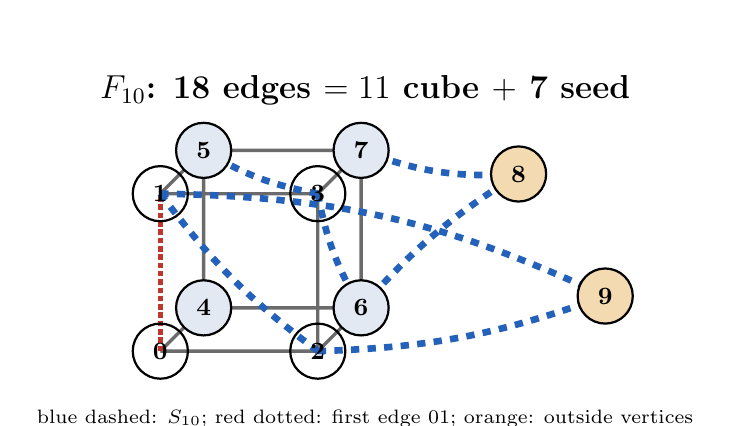
\begin{tikzpicture}[x=1cm,y=1cm,>=Latex]
  \tikzset{
    v/.style={circle,draw=black,thick,minimum size=7mm,inner sep=0pt,font=\small\bfseries},
    back/.style={v,fill=facegray}, outside/.style={v,fill=outsideorange},
    core/.style={draw=black!58,line width=1.2pt},
    seed/.style={draw=seedblue,line width=2.4pt,dashed},
    marked/.style={draw=markedred,line width=2.0pt,densely dotted},
  }
  \coordinate (v0) at (0,0); \coordinate (v1) at (0,2);
  \coordinate (v2) at (2,0); \coordinate (v3) at (2,2);
  \coordinate (v4) at (0.55,0.55); \coordinate (v5) at (0.55,2.55);
  \coordinate (v6) at (2.55,0.55); \coordinate (v7) at (2.55,2.55);
  \coordinate (v8) at (4.55,2.25); \coordinate (v9) at (5.65,0.70);

  \draw[core] (v0)--(v2) (v0)--(v4) (v1)--(v3) (v1)--(v5)
              (v2)--(v3) (v2)--(v6) (v3)--(v7)
              (v4)--(v5) (v4)--(v6) (v5)--(v7) (v6)--(v7);
  \draw[marked] (v0)--(v1);

  \draw[seed] (v1) to[bend right=8] (v2);
  \draw[seed] (v1) to[bend left=12] (v9);
  \draw[seed] (v2) to[bend right=9] (v9);
  \draw[seed] (v3) to[bend left=10] (v5);
  \draw[seed] (v3) to[bend right=10] (v6);
  \draw[seed] (v6) to[bend left=8] (v8);
  \draw[seed] (v7) to[bend right=12] (v8);

  \node[v] at (v0) {0}; \node[v] at (v1) {1};
  \node[v] at (v2) {2}; \node[v] at (v3) {3};
  \node[back] at (v4) {4}; \node[back] at (v5) {5};
  \node[back] at (v6) {6}; \node[back] at (v7) {7};
  \node[outside] at (v8) {8}; \node[outside] at (v9) {9};

  \node[font=\large\bfseries,anchor=south] at (2.6,3.0) {$F_{10}$: 18 edges $=11$ cube $+$ 7 seed};
  \node[font=\scriptsize,anchor=north] at (2.6,-0.62) {blue dashed: $S_{10}$; red dotted: first edge $01$; orange: outside vertices};
\end{tikzpicture}
}
\caption{The $n=10$ upper-bound certificate. The canonical cube is on vertices $0$--$7$; vertices $8$ and $9$ are outside the cube.}
\label{fig:n10seed}
\end{figure}

\subsection{A structural activation lemma}
The early part of the certificate has a simple interpretation.

\begin{lemma}[Twin activation]\label{lem:twin}
Let $Q\cong Q_3$ be a copy in a current graph, let $v\in V(Q)$ have neighbours $a,b,c$ in $Q$, and let $x\notin V(Q)$. If $xa$ and $xb$ are already present, then $xc$ is legal.
\end{lemma}

\begin{proof}
The graph obtained from $Q$ by deleting $v$ and inserting $x$, with $x$ adjacent to $a,b,c$, is isomorphic to $Q_3$: it is the cube obtained by replacing the vertex $v$ by a vertex with the same three neighbours. The nine edges of $Q-v$ remain present and the three edges $xa,xb,xc$ form the three edges incident with $x$. Thus adding $xc$ completes a cube.
\end{proof}

In the $n=10$ seed, $19$ and $29$ are present initially. Applying Lemma~\ref{lem:twin} with $v=0$, whose cube neighbours are $1,2,4$, gives $49$. Applying it with $v=3$, whose cube neighbours are $1,2,7$, gives $79$. The displayed certificate also creates $39$ immediately after $01$; this edge is not required for the activations $49$, $79$, and $07$.

Once $01$, $19$, $29$, and $49$ are present, the cube with vertex map
\[
(0,1,2,3,4,5,6,7)\longmapsto(0,7,1,3,4,6,9,2)
\]
has edge set
\[
\{01,04,07,13,19,23,26,29,37,46,49,67\}.
\]
All edges other than $07$ are then present, so $07$ is legal. Thus the first structural activation can be ordered as
\[
01,\ 39,\ 49,\ 79,\ 07.
\]

The edge $07$ has the following three relevant cube switches:
\[
\begin{aligned}
C_1&=C-\{01,67\}+\{07,16\},\\
C_2&=C-\{02,57\}+\{07,25\},\\
C_3&=C-\{04,37\}+\{07,34\}.
\end{aligned}
\tag{5.3}
\]
Each $C_i$ is a copy of $Q_3$. Explicit cube maps from the canonical cube are, respectively,
\[
(0,1,2,3,4,5,6,7)\mapsto(1,6,3,2,5,4,7,0),
\]
\[
(0,1,2,3,4,5,6,7)\mapsto(2,5,3,1,6,4,7,0),
\]
and
\[
(0,1,2,3,4,5,6,7)\mapsto(3,4,1,5,2,6,0,7).
\]
The first map replaces the cube edges $01,67$ by $07,16$; the second replaces $02,57$ by $07,25$; and the third replaces $04,37$ by $07,34$. Once $07$ is present, each switch has exactly one absent edge, so $16$, $25$, and $34$ are legal in succession. The remaining edges on the eight cube vertices then follow from the certificate rounds.

\begin{figure}[t]
\centering
\resizebox{0.96\linewidth}{!}{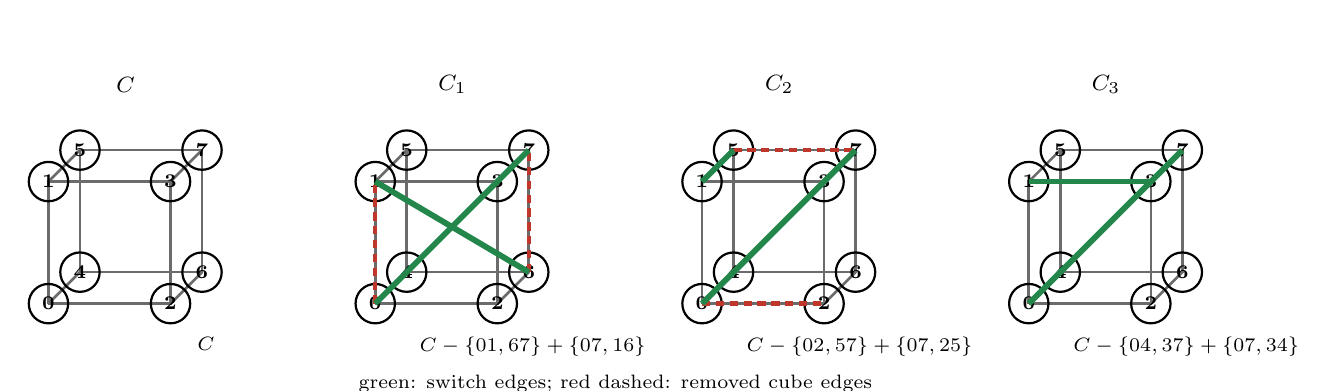
\begin{tikzpicture}[x=1cm,y=1cm]
  \tikzset{
    v/.style={circle,draw=black,thick,minimum size=5mm,inner sep=0pt,font=\scriptsize\bfseries},
    core/.style={draw=black!58,line width=0.95pt},
    gone/.style={draw=markedred,line width=1.6pt,densely dashed},
    add/.style={draw=activationgreen,line width=2.1pt},
    qlab/.style={font=\footnotesize\bfseries,align=center},
  }
  \foreach \sx/\lab in {0/$C$,4.15/$C_1$,8.30/$C_2$,12.45/$C_3$} {
    \begin{scope}[shift={(\sx,0)}]
      \coordinate (a0) at (0,0); \coordinate (a1) at (0,1.55);
      \coordinate (a2) at (1.55,0); \coordinate (a3) at (1.55,1.55);
      \coordinate (a4) at (0.40,0.40); \coordinate (a5) at (0.40,1.95);
      \coordinate (a6) at (1.95,0.40); \coordinate (a7) at (1.95,1.95);
      \draw[core] (a0)--(a1)--(a3)--(a2)--(a0);
      \draw[core] (a4)--(a5)--(a7)--(a6)--(a4);
      \draw[core] (a0)--(a4) (a1)--(a5) (a2)--(a6) (a3)--(a7);
      \node[v] at (a0) {0}; \node[v] at (a1) {1}; \node[v] at (a2) {2}; \node[v] at (a3) {3};
      \node[v] at (a4) {4}; \node[v] at (a5) {5}; \node[v] at (a6) {6}; \node[v] at (a7) {7};
      \node[qlab] at (0.98,2.78) {\lab};
    \end{scope}
  }

  % C_1: remove 01,67; add 07,16
  \begin{scope}[shift={(4.15,0)}]
    \draw[gone] (0,0)--(0,1.55);
    \draw[gone] (1.95,0.40)--(1.95,1.95);
    \draw[add] (0,0)--(1.95,1.95);
    \draw[add] (0,1.55)--(1.95,0.40);
  \end{scope}
  % C_2: remove 02,57; add 07,25
  \begin{scope}[shift={(8.30,0)}]
    \draw[gone] (0,0)--(1.55,0);
    \draw[gone] (0.40,1.95)--(1.95,1.95);
    \draw[add] (0,0)--(1.95,1.95);
    \draw[add] (0,1.55)--(0.40,1.95);
  \end{scope}
  % C_3: remove 04,37; add 07,34
  \begin{scope}[shift={(12.45,0)}]
    \draw[gone] (0,0)--(0.40,0.40);
    \draw[gone] (1.55,1.55)--(1.95,1.95);
    \draw[add] (0,0)--(1.95,1.95);
    \draw[add] (1.55,1.55)--(0,1.55);
  \end{scope}

  \node[font=\scriptsize,anchor=north] at (2.0,-0.30) {$C$};
  \node[font=\scriptsize,anchor=north] at (6.15,-0.30) {$C-\{01,67\}+\{07,16\}$};
  \node[font=\scriptsize,anchor=north] at (10.30,-0.30) {$C-\{02,57\}+\{07,25\}$};
  \node[font=\scriptsize,anchor=north] at (14.45,-0.30) {$C-\{04,37\}+\{07,34\}$};
  \node[font=\scriptsize,anchor=north] at (7.2,-0.78) {green: switch edges; red dashed: removed cube edges};
\end{tikzpicture}
}
\caption{The three cube switches used after $07$ appears. In each panel the green edge is the added edge; red dashed edges are the two cube edges replaced by the switch.}
\label{fig:switches}
\end{figure}

\subsection{Closure layers}
The closure of $S_{10}$ has three closure layers beyond the seed:
\[
\begin{array}{c|l}
\text{round}&\text{edges activated}\\ \hline
0&12,19,29,35,36,68,78\\
1&39,49,79\\
2&03,07,14,16,17,24,25,27,34\\
3&05,06,08,09,18,28,38,47,48,56,58,59,69,89.
\end{array}
\tag{5.4}
\]
An edge in round $r$ depends only on edges in rounds at most $r-1$, so any ordering within one round is legal. This gives a direct round-by-round verification of the certificate closure.

\subsection{Lower bound}
Here
\[
|U_{10}|=\binom{10}{2}-12=33.
\]
To prove $\wsat(K_{10},Q_3)\ge18$, it suffices to exclude six-edge seeds: by Lemma~\ref{lem:mono}, every percolating seed of size at most $6$ would extend to a percolating six-edge seed.

There are
\[
\binom{33}{6}=1,107,568
\]
six-edge seeds. The enumeration canonicalizes each seed under the order-$8$ group $\Gamma_{10}$. By Lemma~\ref{lem:equiv}, two seeds in the same orbit have identical closure size, so one representative per orbit suffices. The resulting complete set has exactly
\[
146,131
\]
representatives. None percolates; the maximum closure contains $25$ of the $33$ outside edges.

\begin{proposition}\label{prop:n10lower}
No six-edge subset of $U_{10}$ percolates. Hence $\sigma_{10}\ge7$.
\end{proposition}

\begin{proof}
The enumeration contains one representative from every $\Gamma_{10}$-orbit of six-edge subsets. Lemma~\ref{lem:equiv} preserves percolation across each orbit. The exact closure routine returns fewer than $33$ outside edges for every representative. Therefore no six-edge seed percolates.
\end{proof}

\begin{theorem}\label{thm:n10}
\[
\boxed{\wsat(K_{10},Q_3)=18.}
\]
\end{theorem}

\begin{proof}
The proposition gives $\sigma_{10}\ge7$ and hence $\wsat(K_{10},Q_3)\ge18$. Proposition~\ref{prop:n10upper} gives the reverse inequality.
\end{proof}

\section{\texorpdfstring{The exact value at $n=11$}{The exact value at n=11}}\label{sec:n11}

\subsection{Upper bound}
The eight-edge seed is
\[
S_{11}=\{35,38,48,68,7\,10,89,3\,10,9\,10\}.
\tag{6.1}
\]
Together with $C-01$, it gives $19$ initial edges. A legal addition order is
\[
\begin{array}{cccccccccc}
01,&08,&25,&07,&09,&16,&18,&03,&05,&06,\\
0\,10,&12,&14,&17,&19,&1\,10,&24,&27,&28,&29,\\
2\,10,&34,&36,&39,&47,&49,&4\,10,&56,&58,&59,\\
5\,10,&69,&6\,10,&78,&79,&8\,10.
\end{array}
\tag{6.2}
\]

\begin{proposition}\label{prop:n11upper}
The graph defined by (6.1) is weakly $Q_3$-saturated in $K_{11}$. Hence
\[
\wsat(K_{11},Q_3)\le19.
\]
\end{proposition}

\begin{proof}
Lemma~\ref{lem:certificate} applies to the order (6.2). For every listed edge $e_i$, the witness table gives an injective map $\phi_i:V(Q_3)\to V(K_{11})$ taking $01$ to $e_i$ and taking every other cube edge to an initially present edge or an edge $e_j$ with $j<i$. Hence each addition creates a copy of $Q_3$. The $36$ additions exhaust the edges missing from the $19$-edge initial graph, so the terminal graph is $K_{11}$.
\end{proof}

\begin{figure}[t]
\centering
\resizebox{0.72\linewidth}{!}{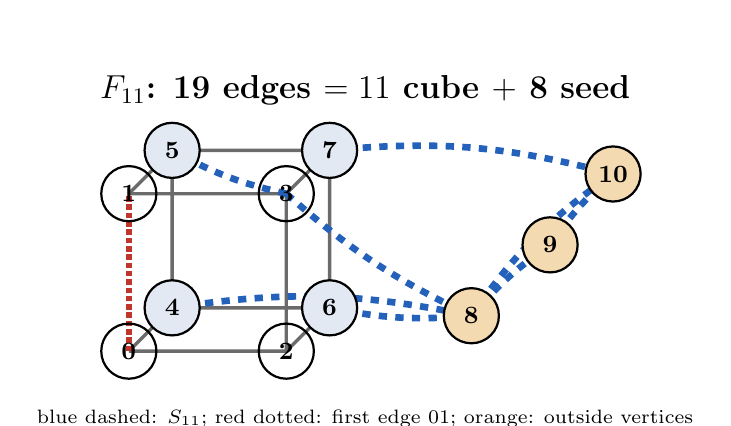
\begin{tikzpicture}[x=1cm,y=1cm,>=Latex]
  \tikzset{
    v/.style={circle,draw=black,thick,minimum size=7mm,inner sep=0pt,font=\small\bfseries},
    back/.style={v,fill=facegray}, outside/.style={v,fill=outsideorange},
    core/.style={draw=black!58,line width=1.2pt},
    seed/.style={draw=seedblue,line width=2.4pt,dashed},
    marked/.style={draw=markedred,line width=2.0pt,densely dotted},
  }
  \coordinate (v0) at (0,0); \coordinate (v1) at (0,2);
  \coordinate (v2) at (2,0); \coordinate (v3) at (2,2);
  \coordinate (v4) at (0.55,0.55); \coordinate (v5) at (0.55,2.55);
  \coordinate (v6) at (2.55,0.55); \coordinate (v7) at (2.55,2.55);
  \coordinate (v8) at (4.35,0.45); \coordinate (v9) at (5.35,1.35); \coordinate (v10) at (6.15,2.25);

  \draw[core] (v0)--(v2) (v0)--(v4) (v1)--(v3) (v1)--(v5)
              (v2)--(v3) (v2)--(v6) (v3)--(v7)
              (v4)--(v5) (v4)--(v6) (v5)--(v7) (v6)--(v7);
  \draw[marked] (v0)--(v1);

  \draw[seed] (v3) to[bend left=8] (v5);
  \draw[seed] (v3) to[bend right=8] (v8);
  \draw[seed] (v4) to[bend left=10] (v8);
  \draw[seed] (v6) to[bend right=8] (v8);
  \draw[seed] (v7) to[bend left=10] (v10);
  \draw[seed] (v8) to[bend left=7] (v9);
  \draw[seed] (v8) to[bend left=10] (v10);
  \draw[seed] (v9) to[bend left=7] (v10);

  \node[v] at (v0) {0}; \node[v] at (v1) {1};
  \node[v] at (v2) {2}; \node[v] at (v3) {3};
  \node[back] at (v4) {4}; \node[back] at (v5) {5};
  \node[back] at (v6) {6}; \node[back] at (v7) {7};
  \node[outside] at (v8) {8}; \node[outside] at (v9) {9}; \node[outside] at (v10) {10};

  \node[font=\large\bfseries,anchor=south] at (3.0,3.0) {$F_{11}$: 19 edges $=11$ cube $+$ 8 seed};
  \node[font=\scriptsize,anchor=north] at (3.0,-0.62) {blue dashed: $S_{11}$; red dotted: first edge $01$; orange: outside vertices};
\end{tikzpicture}
}
\caption{The $n=11$ upper-bound certificate. The orange vertices $8,9,10$ lie outside the canonical cube.}
\label{fig:n11seed}
\end{figure}

\subsection{Lower bound and orbit generation}
For $n=11$,
\[
|U_{11}|=\binom{11}{2}-12=43.
\]
A bound of $18$ would require a percolating seed of size at most $7$. By Lemma~\ref{lem:mono}, any percolating seed of size at most $7$ would extend to a percolating seven-edge seed. It therefore suffices to exclude seven-edge seeds. The raw number of seven-edge seeds is
\[
\binom{43}{7}=32,224,114.
\]
The group $\Gamma_{11}$ has order $24$. The six-edge orbit layer contains $300,563$ representatives. Applying Lemma~\ref{lem:layer} to that layer produces $11,120,831$ seven-edge candidates before canonical deduplication and exactly
\[
1,498,208
\]
representatives afterwards.

\begin{proposition}\label{prop:n11lower}
No seven-edge subset of $U_{11}$ percolates. Hence $\sigma_{11}\ge8$.
\end{proposition}

\begin{proof}
Start with the complete set of $\Gamma_{11}$-orbit representatives at size $6$. Lemma~\ref{lem:layer} shows that adjoining every possible new edge and canonicalizing yields a complete set of orbit representatives at size $7$. There are $11,120,831$ generated children before deduplication and $1,498,208$ representatives afterwards. By Lemma~\ref{lem:equiv}, closure size is constant on each orbit. Algorithm~\ref{alg:closure} gives no full closure among these representatives; the largest terminal closure has $33$ of the $43$ outside edges. Hence no seven-edge seed percolates.
\end{proof}

\subsection{Burnside verification of the orbit counts}\label{sec:burnside}
For an element $g\in\Gamma_{11}$ acting on $U_{11}$ with cycle type
\[
1^{a_1}2^{a_2}3^{a_3}6^{a_6},
\]
the number of fixed $k$-subsets is
\[
\operatorname{Fix}_k(g)
=[x^k](1+x)^{a_1}(1+x^2)^{a_2}(1+x^3)^{a_3}(1+x^6)^{a_6}.
\tag{6.3}
\]
The full cycle-type calculation is Appendix~\ref{app:burnside}. Its aggregate values are
\[
\sum_{g\in\Gamma_{11}}\operatorname{Fix}_6(g)=7,213,512,
\]
\[
\sum_{g\in\Gamma_{11}}\operatorname{Fix}_7(g)=35,956,992.
\]
Burnside's lemma therefore gives
\[
|X_6/\Gamma_{11}|=\frac{7,213,512}{24}=300,563,
\tag{6.4}
\]
and
\[
|X_7/\Gamma_{11}|=\frac{35,956,992}{24}=1,498,208.
\tag{6.5}
\]
These values agree with the orbit-generation counts used in the lower-bound search.

\begin{theorem}\label{thm:n11}
\[
\boxed{\wsat(K_{11},Q_3)=19.}
\]
\end{theorem}

\begin{proof}
The lower-bound proposition gives $\sigma_{11}\ge8$, hence $\wsat(K_{11},Q_3)\ge19$. Proposition~\ref{prop:n11upper} gives the reverse inequality.
\end{proof}

\section{A general extension bound}\label{sec:extension}
The following construction is standard and appears in this form in Terekhov and Zhukovskii \cite{TZ2025}.

\begin{proposition}[Clique extension]\label{prop:extension}
For every $n\ge8$,
\[
\wsat(K_{n+1},Q_3)\le \wsat(K_n,Q_3)+2.
\tag{7.1}
\]
\end{proposition}

\begin{proof}
Let $F$ be weakly $Q_3$-saturated in $K_n$, and let $x$ be a new vertex.
Choose distinct $a,b\in V(F)$ and include $xa$ and $xb$ initially. First follow
a legal order taking $F$ to $K_n$ on the old vertex set. Fix
$y\in V(F)\setminus\{a,b\}$. Since $n\ge8$, four further old vertices can be
chosen distinct from $a,b,y$. In the completed old clique choose a copy
$Q\cong Q_3$ containing a vertex $v$ whose neighbours are $a,b,y$ and whose
remaining four vertices are chosen arbitrarily from those four vertices.
Replacing $v$ by $x$ gives a cube whose three edges incident with $x$ are
$xa,xb,xy$. The first two are present and the other nine cube edges lie in the
completed old clique. Lemma~\ref{lem:twin} therefore makes $xy$ legal. Repeating
for every $y\in V(F)\setminus\{a,b\}$ completes all edges incident with $x$.
Exactly two edges incident with $x$ were initially present, so (7.1) follows.
This is the $Q_3$ specialization of the extension construction in
Terekhov and Zhukovskii~\cite{TZ2025}.
\end{proof}

\begin{corollary}\label{cor:family}
From $\wsat(K_{11},Q_3)=19$,
\[
\boxed{\wsat(K_n,Q_3)\le2n-3\qquad(n\ge11).}
\tag{7.2}
\]
\end{corollary}

\begin{proof}
Apply Proposition~\ref{prop:extension} repeatedly. Each added vertex costs two initial edges.
\end{proof}

The sequence of exact values obtained here is therefore
\[
\begin{array}{c|cccc}
n&8&9&10&11\\ \hline
\wsat(K_n,Q_3)&15&16&18&19\\
\end{array}
\tag{7.3}
\]
where the $n=8$ value is reproduced by the independent sanity check in the supplementary folder. The increments from $n=8$ to $11$ are $1,2,1$.

\section{Analytic perspective}\label{sec:analytic}
The exact lower bound at $n=9$ is a finite exhaustive statement. The invariant in (2.3) also gives finite lower bounds through Theorem~2.1 of \cite{TZ2025}. The values $g^*(1),g^*(2),g^*(3)$ are given explicitly in (2.6), so that
\[
\wsat(K_9,Q_3)\ge13,\qquad
\wsat(K_{10},Q_3)\ge15,\qquad
\wsat(K_{11},Q_3)\ge17.
\]
The asymptotic coefficient obtained from the same invariant is $11/7$ in (2.7); the finite computations here improve these analytic bounds by $3$, $3$, and $2$, respectively.

A direct linear-algebraic proof of $\sigma_9\ge5$ would require a vector assignment to the $24$ outside edges for which every cube implication is represented by a linear dependence. In a formulation adapted to the closure system, one seeks vectors $w_e$ such that, whenever $M$ is a nonempty outside-edge mask of a cube and $e\in M$,
\[
w_e\in\operatorname{span}\{w_f:f\in M\setminus\{e\}\}.
\]
A span of dimension at least $5$ would imply that every percolating seed has at least five edges. No such representation is established here. The limitations of the direct weak-saturation rank method for general graphs are established in \cite{TZrank2025}.

The combinatorial lower-bound framework of Terekhov and Zhukovskii supplies the analytic slope bound in (2.7). Obtaining a direct finite inequality at $n=9$ that reaches $16$ remains a natural problem for further work.

\section{Verification architecture and reproducibility}\label{sec:repro}
The finite lower-bound computations use the complete implication system of
Section~\ref{sec:maskenumeration}. Each edge of $U_n$ is assigned an index. In
the bit-mask implementation, a seed or closure is an integer with one bit per
outside edge. A rule $A\to e$ is stored as an antecedent bit mask, a target
index, and an incidence list for the edges of $A$. When an edge enters the
closure, the counters of the rules containing that edge are incremented. A
rule is fired exactly when its counter reaches $|A|$. Because each edge enters
at most once, the queue performs a finite number of successful insertions, and
Lemma~\ref{lem:closure} identifies the resulting set with the mathematical
closure.

Canonicalization evaluates the action of every element of the finite group
$\Gamma_n$ on the incidence mask and selects the least resulting mask. By
Lemma~\ref{lem:can}, equality of canonical masks is equivalent to membership
in the same orbit. Algorithm~\ref{alg:orbits} therefore generates every orbit
at the next seed size.

The independent $n=9$ Go implementation stores endpoint pairs explicitly and
represents rule antecedents as sorted edge lists. It uses a queue of newly
active edges and recomputes the same closure relation without the bit-mask
state representation of the primary C++ verifier.

Certificate discovery uses a fixed-cardinality local search on subsets of $U_n$. A move exchanges one seed edge with one edge outside the seed and recomputes the exact closure; the score is the closure size. The implementation also uses simulated annealing with random restarts. Each candidate seed is subjected to the explicit witness-map verifier before it is used as an upper-bound certificate. The heuristic search is not used in the lower-bound arguments.

For $n=9$, the primary lower-bound verifier is written in C++ and uses integer bit masks for the $24$ outside edges. The independent lower-bound verifier is written in Go and uses explicit sorted edge lists and adjacency-style rule indexing. The graph-level certificate checker is written in Python and enumerates the $7,560$ labelled cubes as edge sets. Thus the $n=9$ lower bound and the $n=9$ upper-bound certificate are checked by implementations with different data structures and independent code paths.

For $n=10$, the exact orbit search tests all $146,131$ representatives of
six-edge subsets under $\Gamma_{10}$. A separately implemented recheck
reconstructs the orbit layer and closure relation independently and returns
the same representative count and no percolating seed. Separate Python and
C++ programs verify the upper-bound certificate. For $n=11$, the seven-edge orbit layer is generated from the six-edge layer, canonicalized under $\Gamma_{11}$, and then tested by the C++ closure routine. The Burnside calculation is implemented independently in Python.

\begin{table}[t]
\centering
\caption{Finite lower-bound searches. The $n=9$ scan evaluates all labelled
seeds; the orbit count is included for comparison.}
\label{tab:searches}
\begin{tabular}{lrrrrr}
\toprule
$n$ & $|U_n|$ & seed size & seeds evaluated & orbit representatives & percolating \\
\midrule
9  & 24 & 4 & 10,626 & 2,826 & 0 \\
10 & 33 & 6 & 1,107,568 & 146,131 & 0 \\
11 & 43 & 7 & 32,224,114 & 1,498,208 & 0 \\
\bottomrule
\end{tabular}
\end{table}

The corresponding maximum closure sizes are $16$ for the $n=9$ four-edge search, $25$ for the $n=10$ six-edge search, and $33$ for the $n=11$ seven-edge search.

The constructive certificates are independently checked at the graph level by enumerating all labelled copies of $Q_3$ in the corresponding complete host.
\begin{table}[t]
\centering
\caption{Graph-level checks of the three saturation certificates.}
\label{tab:graphcheck}
\begin{tabular}{lrrr}
\toprule
$n$ & $Q_3$ copies checked & initial copies & certificate additions \\
\midrule
9  & 7,560   & 0 & 20 \\
10 & 37,800  & 0 & 27 \\
11 & 138,600 & 0 & 36 \\
\bottomrule
\end{tabular}
\end{table}

\begin{table}[t]
\centering
\caption{Labelled cube copies and distinct outside masks used by the closure system.}
\label{tab:maskcounts}
\begin{tabular}{lrr}
\toprule
$n$ & labelled $Q_3$ copies & distinct outside masks \\
\midrule
9  & 7,560   & 7,122 \\
10 & 37,800  & 36,506 \\
11 & 138,600 & 135,650 \\
\bottomrule
\end{tabular}
\end{table}

The labelled-copy count is the number of explicit cube edge sets checked by
the graph-level verifier. The distinct-mask count is the number of unique
implication masks retained by Algorithm~\ref{alg:masks}; equal masks are
merged because they induce identical closure rules.

All machine-readable certificates, source files, exact execution logs, and hashes are included under \path{supplement/}. The root-level \texttt{README.md} gives the commands for rebuilding the paper and rerunning every theorem-bearing computation. The folder separates manuscript source, theorem-bearing programs, certificates, execution records, and file hashes so that every numerical claim has a corresponding reproducibility record.

\section{Relation to prior work and open problems}\label{sec:open}
The standard clique-extension upper bound gives slope at most $2$ for $Q_3$, while the Terekhov--Zhukovskii invariant gives the asymptotic lower bound $11/7$. The finite values
\[
15,16,18,19
\]
therefore leave a substantial gap between the exact small cases and the known asymptotic lower bound.

The correction at $n=9$ changes the finite picture immediately: the conjectural value $2n-1$ is $17$ at $n=9$, whereas the certificate and exhaustive lower-bound proof give $16$. The same $16$-edge certificate extends to an $18$-edge upper bound at $n=10$, and the $19$-edge $n=11$ certificate improves on the resulting $20$-edge bound.

Several questions remain.

\begin{enumerate}[leftmargin=2em]
\item Determine $\wsat(K_n,Q_3)$ for the next values of $n$, beginning with $n=12$.
\item Determine the asymptotic slope $c_{Q_3}$ in (2.7), currently bounded by $11/7\le c_{Q_3}\le2$.
\item Find structural families that explain the transition from the exceptional finite values to a general upper bound below $2n-3$, or prove that the $2n-3$ family is asymptotically optimal.
\item Develop a sharp analytic lower bound specialized to $Q_3$. In particular, a linear-algebraic or other invariant attaining $16$ at $n=9$ would replace the finite exclusion of all $10,626$ four-edge seeds by a direct inequality.
\end{enumerate}

\section{Conclusion}
The exact values are
\[
\boxed{\wsat(K_9,Q_3)=16,\qquad
\wsat(K_{10},Q_3)=18,\qquad
\wsat(K_{11},Q_3)=19.}
\]
The upper bounds are given by the explicit witness tables, and the lower
bounds by the complete finite closure searches. The $n=11$ construction gives
$\wsat(K_n,Q_3)\le2n-3$ for every $n\ge11$.

\paragraph{Code and data availability.}
Source code, machine-readable certificates, orbit representatives, and
verification records for all computations reported in this paper are
available in the public repository \cite{SahaCode}. The release
\texttt{v1.0.0-paper} is archived at Zenodo under the DOI given in
\cite{SahaCode}.


\newpage

\begingroup\sloppy
\begin{thebibliography}{99}

\bibitem{Bollobas1968}
B.~Bollob\'as,
\newblock Weakly $k$-saturated graphs,
\newblock in \emph{Beitr\"age zur Graphentheorie}, B.~G.~Teubner Verlagsgesellschaft, Leipzig, 1968, pp.~25--31.

\bibitem{Balogh2012}
J.~Balogh, B.~Bollob\'as, R.~Morris, and O.~Riordan,
\newblock Linear algebra and bootstrap percolation,
\newblock \emph{Journal of Combinatorial Theory, Series A} 119 (2012), 1328--1335,
\newblock doi:10.1016/j.jcta.2012.03.005.

\bibitem{MNS2017}
N.~Morrison, J.~A.~Noel, and A.~Scott,
Saturation in the hypercube and bootstrap percolation, \emph{Combinatorics, Probability and Computing} 26 (2017), 78--98, \url{https://doi.org/10.1017/S0963548316000122}.

\bibitem{KMM2021}
G.~Kronenberg, T.~Martins, and N.~Morrison,
\newblock Weak saturation numbers of complete bipartite graphs in the clique,
\newblock \emph{Journal of Combinatorial Theory, Series A} 178 (2021), 105357,
\newblock doi:10.1016/j.jcta.2020.105357.

\bibitem{Alon1985}
N.~Alon,
\newblock An extremal problem for sets with applications to graph theory,
\newblock \emph{Journal of Combinatorial Theory, Series A} 40 (1985), 82--89,
\newblock doi:10.1016/0097-3165(85)90048-2.

\bibitem{TZ2025}
N.~Terekhov and M.~Zhukovskii,
\newblock Weak saturation in graphs: a combinatorial approach,
\newblock \emph{Journal of Combinatorial Theory, Series B} 172 (2025), 146--167,
\newblock doi:10.1016/j.jctb.2024.12.007.

\bibitem{TZrank2025}
N.~Terekhov and M.~Zhukovskii,
\newblock Weak saturation rank: a failure of the linear algebraic approach to weak saturation,
\newblock \emph{Combinatorica} 45 (2025),
\newblock doi:10.1007/s00493-025-00174-y.

\bibitem{PCMI2025}
T.~Trakulthongchai, D.~Xu, and K.~Zhu,
\newblock \emph{Weak saturation number of the 3-cube in the complete graph},
\newblock Park City Mathematics Institute, Summer 2025 project slides,
\newblock \url{https://www.ias.edu/sites/default/files/Trakulthongchai_Xu_Zhu.pdf}.

\bibitem{OPG}
Open Problem Garden,
\newblock \emph{Weak saturation of the cube in the clique}, problem OPG-60013,
\newblock \url{https://www.openproblemgarden.org/op/weak_saturation_of_the_cube_in_the_clique}.

\bibitem{SahaCode}
V.~Saha,
\newblock \emph{Computational materials for Weak Saturation of the 3-Cube in Complete Graphs: Exact Values at Orders 9,10,11},
\newblock version 1.0.0-paper,
\newblock Zenodo, 2026,
\newblock doi:\url{https://doi.org/10.5281/zenodo.23121234}.


\end{thebibliography}
\endgroup

\newpage
\appendix

\section{Complete certificate witness tables}\label{app:witness}
For each certificate, row $i$ records the added edge $e_i$, an injective map
\[
\phi_i=(\phi_i(0),\ldots,\phi_i(7)),
\]
and the earlier certificate steps used by the witness. The canonical cube edge set is
\[
E(Q_3)=\{01,02,04,13,15,23,26,37,45,46,57,67\}.
\]
Thus a row is checked by mapping this edge set through $\phi_i$. The target edge is $\phi_i(0)\phi_i(1)$; the dependency column identifies precisely those witness edges created during the certificate. Every other witness edge is initial.

\subsection*{$n=9$}
\begingroup\scriptsize
\begin{longtable}{r c p{0.39\textwidth} p{0.28\textwidth}}
\toprule
step & edge & $\phi(0),\ldots,\phi(7)$ & earlier steps used \\*
\midrule
\endfirsthead
\toprule
step & edge & $\phi(0),\ldots,\phi(7)$ & earlier steps used \\*
\midrule
\endhead
\midrule
\multicolumn{4}{r}{\emph{continued on next page}}\\
\endfoot
\bottomrule
\endlastfoot
1 & \texttt{01} & $(0,\,1,\,2,\,3,\,4,\,5,\,6,\,7)$ & - \\
2 & \texttt{14} & $(1,\,4,\,0,\,5,\,2,\,6,\,3,\,7)$ & 1 \\
3 & \texttt{48} & $(4,\,8,\,5,\,0,\,6,\,2,\,7,\,3)$ & - \\
4 & \texttt{78} & $(7,\,8,\,3,\,2,\,5,\,4,\,0,\,1)$ & 1,\,2,\,3 \\
5 & \texttt{06} & $(0,\,6,\,3,\,2,\,5,\,4,\,7,\,8)$ & 3,\,4 \\
6 & \texttt{16} & $(1,\,6,\,3,\,2,\,5,\,4,\,0,\,8)$ & 3 \\
7 & \texttt{17} & $(1,\,7,\,2,\,3,\,4,\,5,\,6,\,0)$ & 2,\,5 \\
8 & \texttt{18} & $(1,\,8,\,3,\,2,\,5,\,4,\,0,\,6)$ & 3,\,5 \\
9 & \texttt{24} & $(2,\,4,\,3,\,1,\,6,\,0,\,7,\,5)$ & 2,\,5 \\
10 & \texttt{25} & $(2,\,5,\,3,\,1,\,6,\,4,\,0,\,8)$ & 3,\,5,\,8 \\
11 & \texttt{27} & $(2,\,7,\,1,\,3,\,4,\,5,\,6,\,0)$ & 5,\,6,\,9 \\
12 & \texttt{34} & $(3,\,4,\,1,\,6,\,2,\,5,\,8,\,0)$ & 5,\,6,\,8,\,10 \\
13 & \texttt{35} & $(3,\,5,\,4,\,0,\,7,\,1,\,2,\,6)$ & 5,\,6,\,7,\,9,\,11,\,12 \\
14 & \texttt{36} & $(3,\,6,\,4,\,1,\,5,\,0,\,2,\,8)$ & 2,\,5,\,6,\,8,\,9,\,10,\,12,\,13 \\
15 & \texttt{38} & $(3,\,8,\,4,\,1,\,5,\,0,\,2,\,6)$ & 2,\,5,\,6,\,8,\,9,\,10,\,12,\,13 \\
16 & \texttt{47} & $(4,\,7,\,3,\,2,\,5,\,1,\,0,\,6)$ & 5,\,6,\,7,\,11,\,12 \\
17 & \texttt{56} & $(5,\,6,\,3,\,1,\,4,\,0,\,2,\,8)$ & 5,\,6,\,8,\,9,\,13 \\
18 & \texttt{58} & $(5,\,8,\,3,\,1,\,4,\,0,\,2,\,6)$ & 5,\,6,\,8,\,9,\,13 \\
19 & \texttt{68} & $(6,\,8,\,2,\,1,\,3,\,0,\,4,\,5)$ & 8,\,9,\,12,\,14 \\
20 & \texttt{07} & $(0,\,7,\,5,\,2,\,6,\,1,\,3,\,4)$ & 2,\,5,\,6,\,7,\,9,\,10,\,11,\,12,\,13,\,14 \\
\end{longtable}

\endgroup

\subsection*{$n=10$}
\begingroup\scriptsize
\begin{longtable}{r c p{0.39\textwidth} p{0.28\textwidth}}
\toprule
step & edge & $\phi(0),\ldots,\phi(7)$ & earlier steps used \\*
\midrule
\endfirsthead
\toprule
step & edge & $\phi(0),\ldots,\phi(7)$ & earlier steps used \\*
\midrule
\endhead
\midrule
\multicolumn{4}{r}{\emph{continued on next page}}\\
\endfoot
\bottomrule
\endlastfoot
1 & \texttt{01} & $(0,\,1,\,2,\,3,\,4,\,5,\,6,\,7)$ & - \\
2 & \texttt{39} & $(3,\,9,\,5,\,1,\,6,\,2,\,4,\,0)$ & 1 \\
3 & \texttt{07} & $(0,\,7,\,1,\,5,\,2,\,6,\,9,\,3)$ & 1,\,2 \\
4 & \texttt{17} & $(1,\,7,\,2,\,0,\,3,\,5,\,6,\,4)$ & 3 \\
5 & \texttt{03} & $(0,\,3,\,2,\,1,\,4,\,5,\,6,\,7)$ & 4 \\
6 & \texttt{25} & $(2,\,5,\,6,\,4,\,9,\,1,\,3,\,0)$ & 1,\,2,\,5 \\
7 & \texttt{47} & $(4,\,7,\,5,\,1,\,6,\,3,\,2,\,0)$ & 1,\,4,\,5,\,6 \\
8 & \texttt{16} & $(1,\,6,\,0,\,2,\,7,\,4,\,3,\,5)$ & 1,\,4,\,5,\,6,\,7 \\
9 & \texttt{27} & $(2,\,7,\,0,\,3,\,5,\,4,\,1,\,6)$ & 1,\,5,\,6,\,7,\,8 \\
10 & \texttt{56} & $(5,\,6,\,1,\,3,\,4,\,7,\,0,\,2)$ & 1,\,7,\,9 \\
11 & \texttt{24} & $(2,\,4,\,0,\,7,\,3,\,6,\,1,\,5)$ & 1,\,3,\,7,\,10 \\
12 & \texttt{34} & $(3,\,4,\,0,\,2,\,6,\,7,\,1,\,5)$ & 1,\,5,\,6,\,7,\,8,\,11 \\
13 & \texttt{05} & $(0,\,5,\,1,\,6,\,2,\,4,\,3,\,7)$ & 1,\,7,\,8,\,10,\,11 \\
14 & \texttt{06} & $(0,\,6,\,1,\,5,\,2,\,4,\,3,\,7)$ & 1,\,7,\,10,\,11 \\
15 & \texttt{14} & $(1,\,4,\,0,\,2,\,5,\,7,\,3,\,6)$ & 1,\,5,\,7,\,11 \\
16 & \texttt{59} & $(5,\,9,\,4,\,2,\,6,\,3,\,1,\,0)$ & 1,\,2,\,5,\,8,\,10,\,11,\,15 \\
17 & \texttt{49} & $(4,\,9,\,5,\,2,\,6,\,3,\,1,\,0)$ & 1,\,2,\,5,\,6,\,8 \\
18 & \texttt{69} & $(6,\,9,\,2,\,4,\,3,\,5,\,0,\,1)$ & 1,\,5,\,11,\,15,\,16,\,17 \\
19 & \texttt{09} & $(0,\,9,\,1,\,4,\,2,\,5,\,3,\,6)$ & 1,\,6,\,10,\,15,\,16,\,17 \\
20 & \texttt{79} & $(7,\,9,\,2,\,4,\,3,\,5,\,0,\,1)$ & 1,\,5,\,9,\,11,\,15,\,16,\,17 \\
21 & \texttt{28} & $(2,\,8,\,0,\,6,\,3,\,7,\,1,\,4)$ & 1,\,7,\,14,\,15 \\
22 & \texttt{58} & $(5,\,8,\,1,\,6,\,2,\,7,\,0,\,3)$ & 1,\,5,\,6,\,8,\,9 \\
23 & \texttt{18} & $(1,\,8,\,0,\,2,\,4,\,6,\,3,\,5)$ & 1,\,5,\,6,\,10,\,12,\,15,\,21 \\
24 & \texttt{38} & $(3,\,8,\,0,\,2,\,5,\,6,\,1,\,4)$ & 1,\,5,\,10,\,11,\,15,\,21 \\
25 & \texttt{48} & $(4,\,8,\,1,\,5,\,2,\,6,\,0,\,3)$ & 1,\,5,\,11,\,15,\,22 \\
26 & \texttt{08} & $(0,\,8,\,1,\,4,\,2,\,5,\,3,\,6)$ & 1,\,6,\,10,\,15,\,22,\,25 \\
27 & \texttt{89} & $(8,\,9,\,2,\,4,\,3,\,5,\,0,\,1)$ & 1,\,5,\,11,\,15,\,16,\,17,\,21,\,24 \\
\end{longtable}

\endgroup

\subsection*{$n=11$}
\begingroup\scriptsize
\begin{longtable}{r c p{0.39\textwidth} p{0.28\textwidth}}
\toprule
step & edge & $\phi(0),\ldots,\phi(7)$ & earlier steps used \\*
\midrule
\endfirsthead
\toprule
step & edge & $\phi(0),\ldots,\phi(7)$ & earlier steps used \\*
\midrule
\endhead
\midrule
\multicolumn{4}{r}{\emph{continued on next page}}\\
\endfoot
\bottomrule
\endlastfoot
1 & \texttt{01} & $(0,\,1,\,2,\,3,\,4,\,5,\,6,\,7)$ & - \\
2 & \texttt{08} & $(0,\,8,\,1,\,3,\,4,\,6,\,5,\,7)$ & 1 \\
3 & \texttt{25} & $(2,\,5,\,0,\,1,\,6,\,7,\,8,\,3)$ & 1,\,2 \\
4 & \texttt{07} & $(0,\,7,\,1,\,3,\,4,\,6,\,5,\,2)$ & 1,\,3 \\
5 & \texttt{09} & $(0,\,9,\,4,\,8,\,7,\,10,\,5,\,3)$ & 4 \\
6 & \texttt{16} & $(1,\,6,\,0,\,4,\,3,\,7,\,2,\,5)$ & 1,\,3 \\
7 & \texttt{18} & $(1,\,8,\,0,\,9,\,5,\,3,\,7,\,10)$ & 1,\,4,\,5 \\
8 & \texttt{03} & $(0,\,3,\,1,\,8,\,2,\,5,\,6,\,4)$ & 1,\,3,\,6,\,7 \\
9 & \texttt{05} & $(0,\,5,\,3,\,2,\,8,\,4,\,1,\,6)$ & 2,\,3,\,6,\,7,\,8 \\
10 & \texttt{06} & $(0,\,6,\,3,\,2,\,8,\,4,\,1,\,5)$ & 2,\,3,\,7,\,8 \\
11 & \texttt{010} & $(0,\,10,\,6,\,7,\,8,\,3,\,1,\,5)$ & 2,\,6,\,7,\,10 \\
12 & \texttt{12} & $(1,\,2,\,0,\,5,\,8,\,6,\,3,\,7)$ & 1,\,3,\,7,\,8,\,9 \\
13 & \texttt{14} & $(1,\,4,\,0,\,5,\,6,\,8,\,2,\,3)$ & 1,\,6,\,9 \\
14 & \texttt{17} & $(1,\,7,\,0,\,3,\,4,\,6,\,5,\,2)$ & 1,\,3,\,8,\,9,\,13 \\
15 & \texttt{19} & $(1,\,9,\,0,\,10,\,6,\,8,\,2,\,3)$ & 1,\,6,\,11 \\
16 & \texttt{110} & $(1,\,10,\,0,\,3,\,6,\,7,\,2,\,5)$ & 1,\,3,\,6,\,8 \\
17 & \texttt{24} & $(2,\,4,\,0,\,5,\,6,\,8,\,1,\,3)$ & 1,\,6,\,9 \\
18 & \texttt{27} & $(2,\,7,\,0,\,3,\,4,\,6,\,1,\,8)$ & 1,\,7,\,8,\,13,\,17 \\
19 & \texttt{28} & $(2,\,8,\,0,\,3,\,4,\,6,\,1,\,7)$ & 1,\,8,\,13,\,14,\,17 \\
20 & \texttt{29} & $(2,\,9,\,0,\,1,\,4,\,8,\,5,\,3)$ & 1,\,9,\,15,\,17 \\
21 & \texttt{210} & $(2,\,10,\,0,\,3,\,6,\,7,\,1,\,5)$ & 1,\,6,\,8 \\
22 & \texttt{34} & $(3,\,4,\,0,\,1,\,8,\,6,\,2,\,7)$ & 1,\,8,\,13,\,14,\,18,\,19 \\
23 & \texttt{36} & $(3,\,6,\,0,\,2,\,4,\,8,\,1,\,9)$ & 1,\,8,\,13,\,15,\,20,\,22 \\
24 & \texttt{39} & $(3,\,9,\,0,\,2,\,6,\,8,\,1,\,4)$ & 1,\,6,\,8,\,13,\,17,\,20,\,23 \\
25 & \texttt{47} & $(4,\,7,\,1,\,5,\,2,\,6,\,0,\,3)$ & 1,\,8,\,13,\,17,\,23 \\
26 & \texttt{49} & $(4,\,9,\,1,\,8,\,2,\,10,\,0,\,3)$ & 1,\,7,\,8,\,13,\,17,\,21 \\
27 & \texttt{410} & $(4,\,10,\,1,\,7,\,2,\,9,\,0,\,3)$ & 1,\,8,\,13,\,14,\,17,\,20,\,24 \\
28 & \texttt{56} & $(5,\,6,\,1,\,4,\,3,\,7,\,0,\,2)$ & 1,\,8,\,13,\,17,\,18 \\
29 & \texttt{58} & $(5,\,8,\,1,\,4,\,3,\,6,\,0,\,2)$ & 1,\,8,\,13,\,17,\,23 \\
30 & \texttt{59} & $(5,\,9,\,1,\,4,\,3,\,8,\,0,\,2)$ & 1,\,8,\,13,\,17,\,19,\,26 \\
31 & \texttt{510} & $(5,\,10,\,1,\,4,\,3,\,7,\,0,\,2)$ & 1,\,8,\,13,\,17,\,18,\,27 \\
32 & \texttt{69} & $(6,\,9,\,2,\,4,\,3,\,5,\,0,\,1)$ & 1,\,8,\,13,\,17,\,23,\,26,\,30 \\
33 & \texttt{610} & $(6,\,10,\,2,\,4,\,3,\,5,\,0,\,1)$ & 1,\,8,\,13,\,17,\,23,\,27,\,31 \\
34 & \texttt{78} & $(7,\,8,\,2,\,4,\,3,\,5,\,0,\,1)$ & 1,\,8,\,13,\,17,\,18,\,29 \\
35 & \texttt{79} & $(7,\,9,\,2,\,4,\,3,\,5,\,0,\,1)$ & 1,\,8,\,13,\,17,\,18,\,26,\,30 \\
36 & \texttt{810} & $(8,\,10,\,2,\,4,\,3,\,5,\,0,\,1)$ & 1,\,8,\,13,\,17,\,19,\,27,\,31 \\
\end{longtable}

\endgroup

\section{Burnside table}\label{app:burnside}
For $g\in\Gamma_{11}$, let $a_j(g)$ denote the number of $j$-cycles in the
permutation induced by $g$ on the $43$ outside edges. The fixed $k$-subsets
are counted by
\[
\operatorname{Fix}_k(g)=[x^k]
(1+x)^{a_1(g)}(1+x^2)^{a_2(g)}
(1+x^3)^{a_3(g)}(1+x^6)^{a_6(g)}.
\tag{B.1}
\]
The complete calculation is
\[
\begin{array}{c|r|r|r}
\text{cycle type on }U_{11}&\text{multiplicity}&\operatorname{Fix}_6&\operatorname{Fix}_7\\
\hline
1^{43}&1&6,096,454&32,224,114\\
1^{23}2^{10}&3&301,834&1,043,770\\
1^{11}2^{16}&3&12,902&33,682\\
1\,2^{21}&3&1,330&1,330\\
1^{16}3^9&2&13,084&28,396\\
1^6 2^5 3^5 6^2&2&498&862\\
1^2 2^9 3\,6^4&2&74&106\\
2^8 3\,6^4&2&60&28\\
1^3 2^{20}&4&1,710&3,610\\
1^{21}2^{11}&1&131,814&416,734\\
1^5 2^{19}&1&2,774&6,574\\
\midrule
\text{total}&24&7,213,512&35,956,992
\end{array}
\tag{B.2}
\]
Consequently, Burnside's lemma gives
\[
|X_6/\Gamma_{11}|=\frac{7,213,512}{24}=300,563,
\qquad
|X_7/\Gamma_{11}|=\frac{35,956,992}{24}=1,498,208.
\tag{B.3}
\]
The first total equals
$\binom{43}{6}$ after weighting by stabilizers, while the second total
similarly accounts for the $7$-subset action. These orbit counts agree with
the representatives produced by Algorithm~\ref{alg:orbits}.

\section{Finite-search data and verification records}\label{app:records}
The supplementary material contains the executable verification programs, machine-readable certificates, orbit representatives, and execution records used for the finite computations.

\begin{itemize}
\item \textbf{Certificates:} \path{supplement/certificates/} contains the complete machine-readable certificates and witness tables.
\item \textbf{$n=9$ verification:} \path{supplement/programs/n9_exact_verifier.cpp}, \path{n9_independent_lower.go}, and \path{n9_graph_level_check.py} provide distinct verification layers.
\item \textbf{Lower bounds for $n=10,11$:} \path{supplement/programs/n10_lower_orbit_recheck.cpp} and \path{n11_lower_orbit7.cpp}.
\item \textbf{Burnside verification:} \path{supplement/programs/n11_burnside.py}.
\item \textbf{Certificate verification:} Python and C++ verifiers in \path{supplement/programs/}.
\item \textbf{Records and hashes:} \path{logs/} contains execution outputs and \path{SHA256SUMS.txt} contains file hashes.
\end{itemize}

The finite verification specification in \path{PROOF_SPEC.md} records the edge sets, closure rules, orbit actions, certificate conditions, and finite statements used by the verification programs.

\end{document}
